% !TEX root = owasp-doc.tex
% ================================================
%	OVERVIEW
% ================================================
\headerimage
\chapter{Overview}
Every internet user and business should prepare for the impact of a surge in
powerful generative artificial intelligence (GenAI) applications. GenAI holds
enormous promise and opportunities for discovery, efficiency, and driving
corporate growth across many industries and disciplines. However, as with any
strong new technology, it introduces new challenges to security and privacy.

Artificial Intelligence, Machine Learning, Large Language Models, and Diffusion
Models have been in development and the focus of academic research for many
years. Recent improvements in training data availability, computer power,
GenAI capacity, and the release of solutions such as ChatGPT, ElevenLabs,
Midjourney, along with their broader availability outside of what previously
was a relatively isolated and specialized field, have led to its eruptive
growth. These advances in artificial intelligence (AI) emphasize the importance
of organizations developing plans to manage their engagement and use of AI
within their organization.

\begin{itemize}
  \item \textbf{Artificial intelligence} is a broad term that encompasses all fields of
  computer science that enable machines to accomplish tasks that would normally
  require human intelligence. Machine learning and generative AI are two
  subcategories of AI.
  \item \textbf{Machine learning} is a subset of AI that focuses on creating algorithms
  that can learn from data. Machine learning algorithms are trained on a set of
  data, and then they can use that data to make predictions or decisions about
  new data.
  \item \textbf{Generative AI} is a type of machine learning that focuses on creating
  new data. Often, GenAI relies on the use of large language models to perform
  the tasks needed to create the new data.
  \item A \textbf{large language model (LLM)} is a type of AI program that uses machine
  learning to perform natural language processing (NLP) tasks. LLMs are trained
  on large data sets to understand, summarize, generate, and predict new
  content.
\end{itemize}

\clearpage
The diagram below shows the relationship of LLM to the field of AI generally:

\begin{figure}[h]
  \centering
  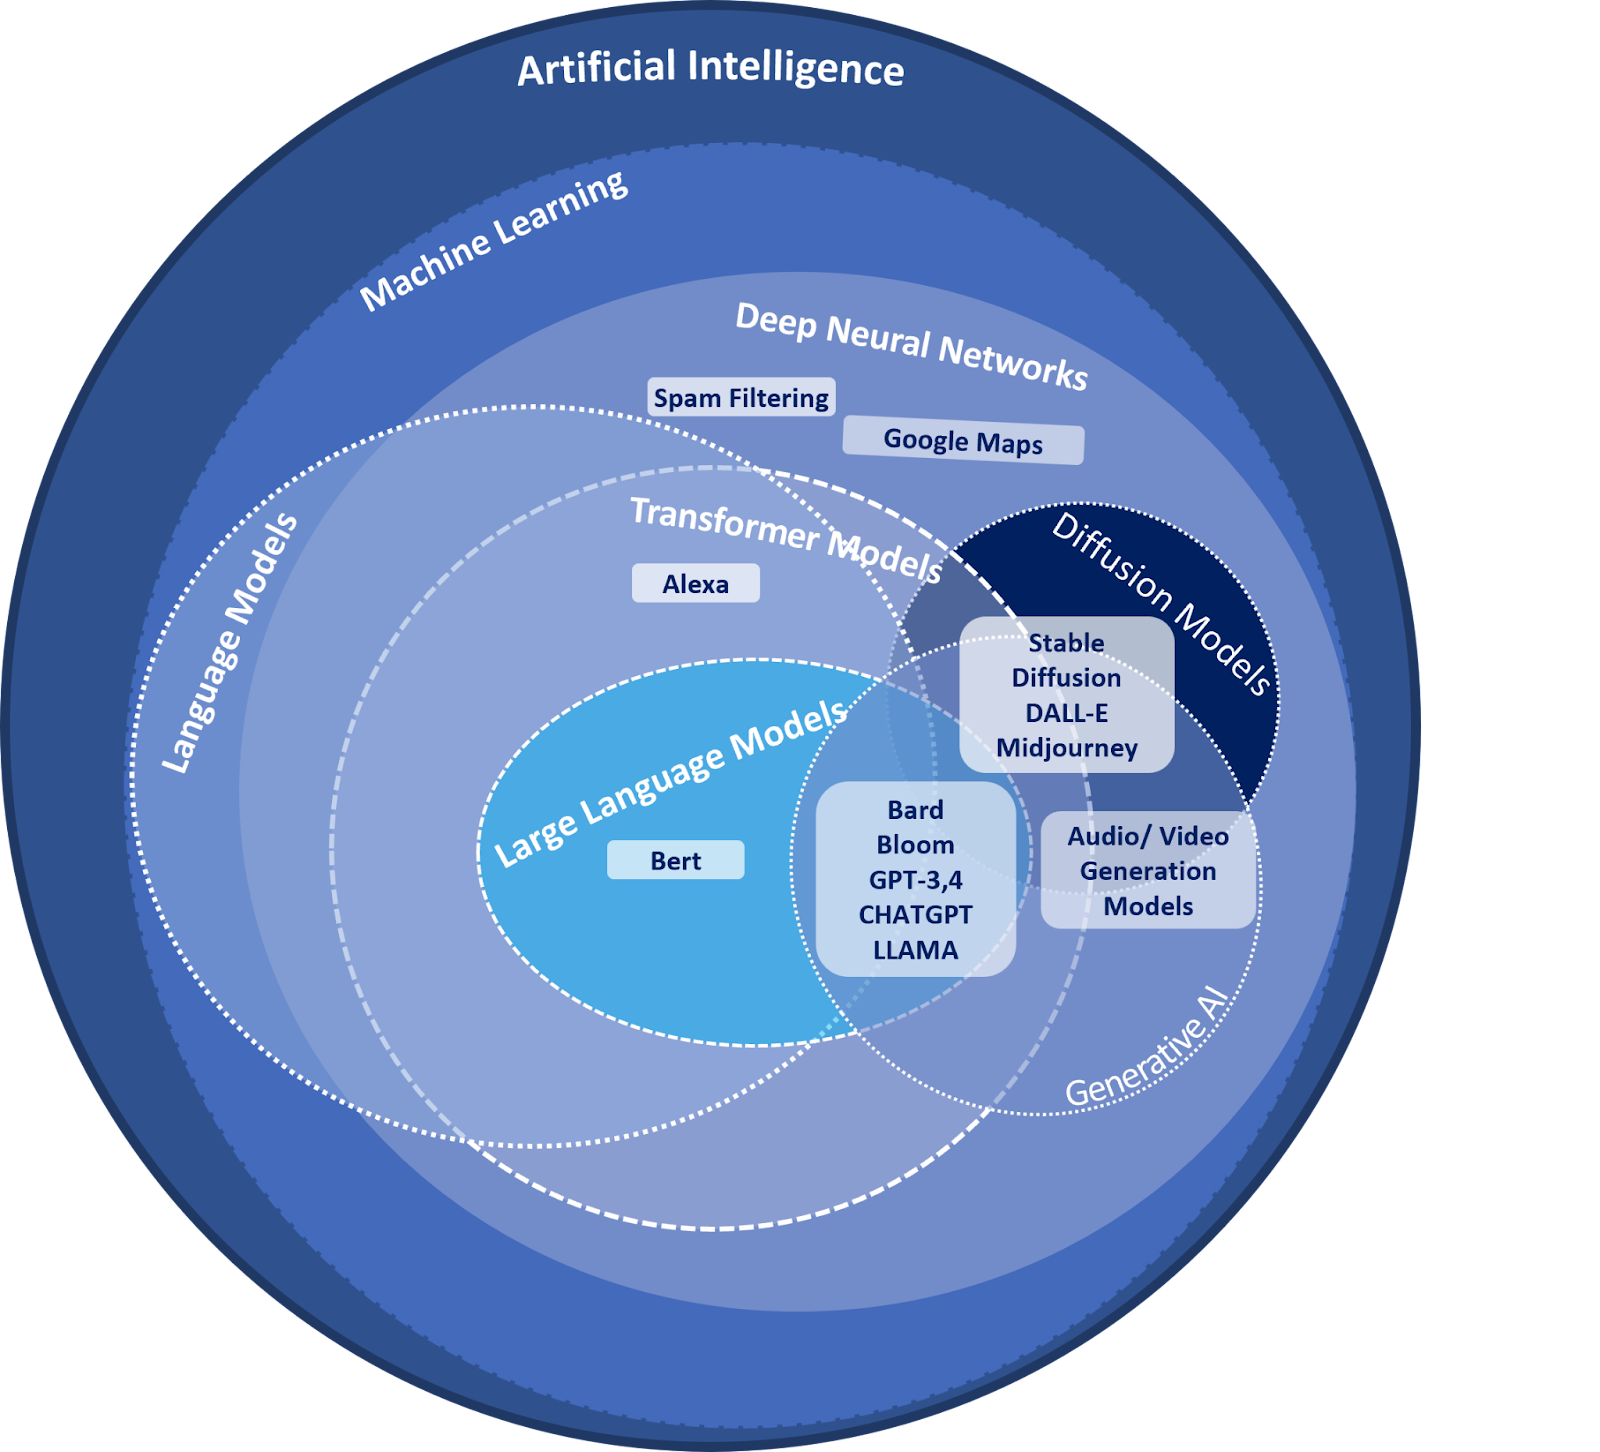
\includegraphics[width=\textwidth]{ai_llm_relationship}
  \caption{Image of LLM relationship within the field of Artificial Intelligence}
  \label{fig:ai-llm-relationship}
\end{figure}

Organizations will face new challenges defending and managing GenAI solutions.
Additionally, there is significant potential for accelerated threats from threat
actors who will use GenAI to augment attack techniques.

Many applications within a business employ artificial intelligence applications,
such as human resource hiring, SPAM detection for email, behavioral analytics
for SIEM, and MDR apps. The primary focus of this document is on Large Language
Model applications, which can produce content.

\clearpage
\section{Responsible and Trustworthy Artificial Intelligence}
As challenges and benefits of Artificial Intelligence emerge - and regulations
and laws are passed - the principles and pillars of responsible and trustworthy
AI usage are evolving from idealistic objects and concerns to established
standards.

The \href{https://owasp.org/www-project-ai-security-and-privacy-guide/}{OWASP AI Security and Privacy Guide}
working group is monitoring these changes and addressing the broader and more
challenging considerations for all aspects of artificial intelligence.

\begin{figure}[h]
  \centering
  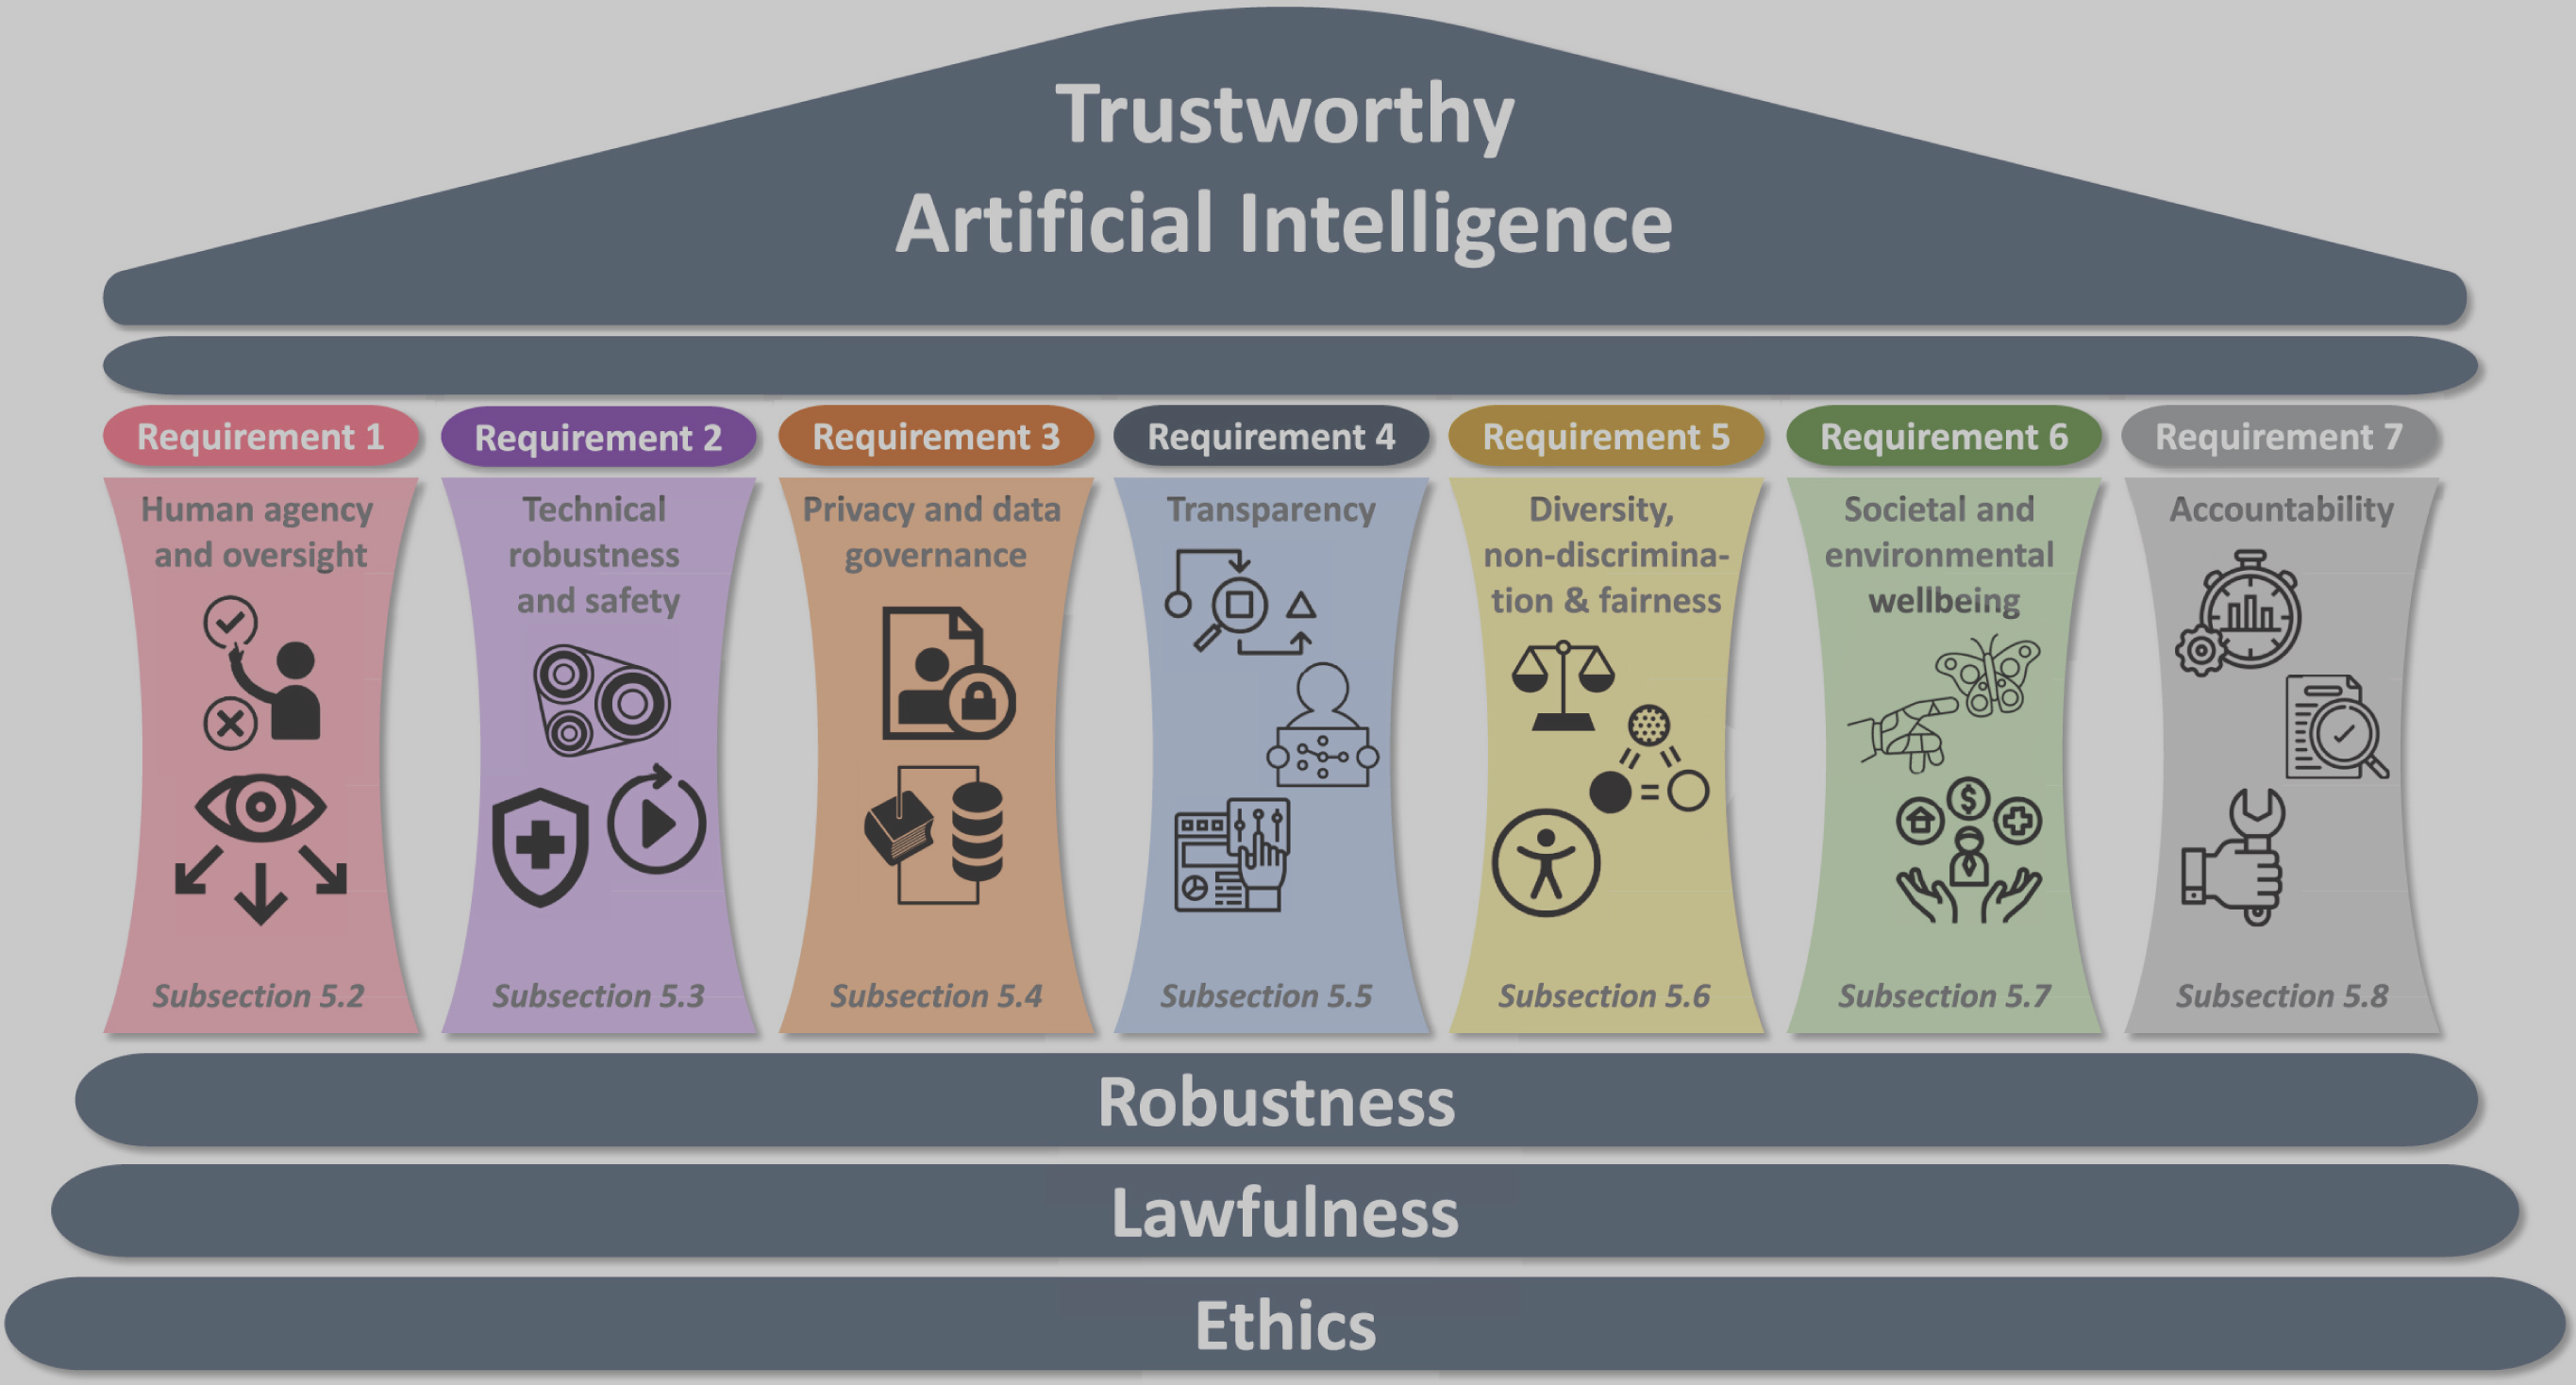
\includegraphics[width=\textwidth]{trustworthy_ai}
  \caption{Image credit \href{https://montrealethics.ai/}{Montreal AI Ethics Institute}}
  \label{fig:trustworthy-ai}
\end{figure}

\clearpage
\section{Who is This For?}
Executive, technology, cybersecurity, privacy, compliance, and legal leaders
must pay close attention to the fast GenAI technological transformation and
devise a strategy to benefit from opportunities while fighting against threats
and managing risks.

This checklist is designed to assist these technology and business leaders in
quickly understanding the risks and benefits of using LLM, allowing them to
focus on developing a comprehensive list of essential areas and tasks required
to defend  and protect the organization as they create a Large Language Model
strategy.

Scenarios presented here include those that pertain to internal use of models
released commercially or those that are open sourced, as well as scenarios for
organizations that consume LLM services provided by third-parties. Resources
from MITRE Engenuity, OWASP, and others are referenced.

The diagram below shows how these resources can be used to create a threat
informed defense strategy.

\begin{figure}[h]
  \centering
  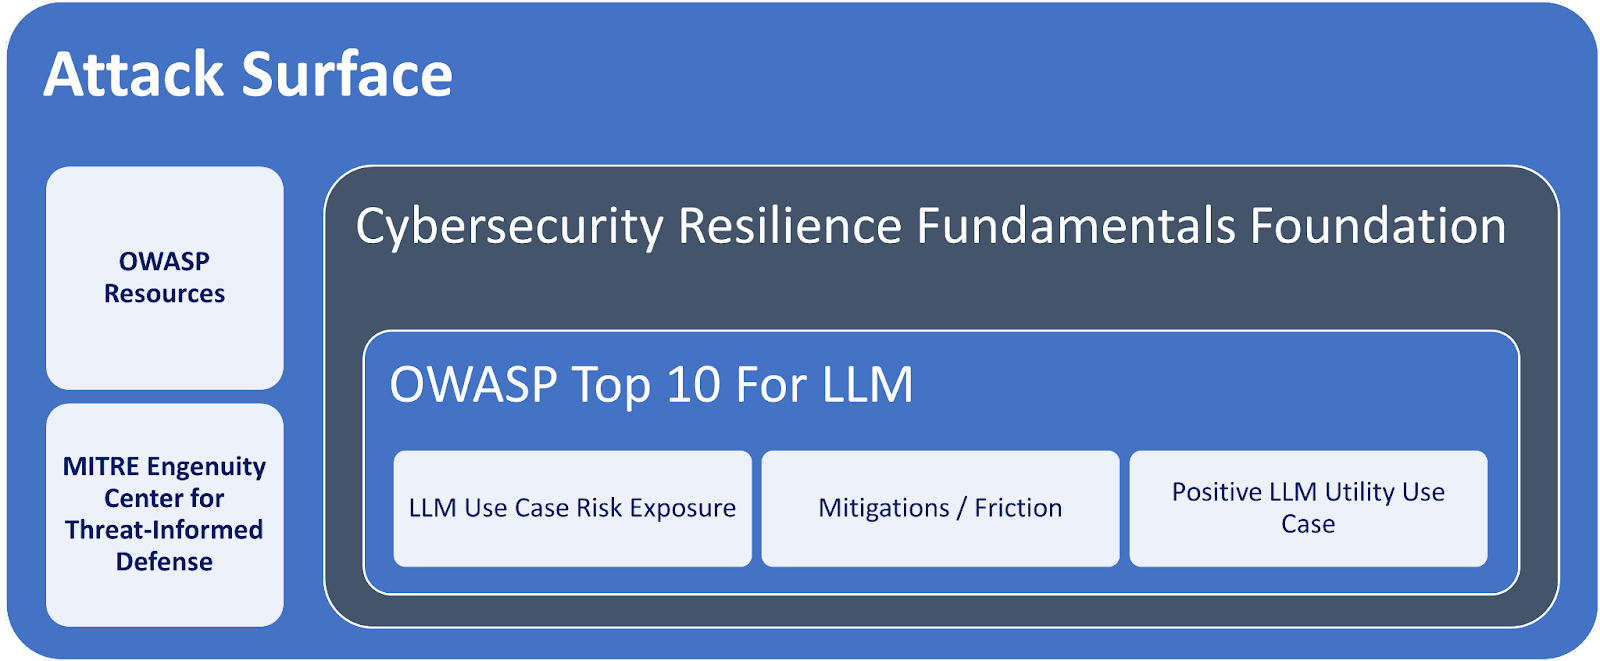
\includegraphics[width=\textwidth]{llm_attack_surface}
  \caption{Image of integrating LLM Security with OWASP and MITRE resources}
  \label{fig:llm-attack-surface}
\end{figure}

It is the hope of the OWASP Top 10 for LLM Applications team that this list will
help organizations improve their existing defensive techniques and develop
techniques to address the new threats that come from using this exciting technology.

\clearpage
\section{Why a Checklist?}

Checklists can help with strategy development by ensuring thoroughness,
clarifying goals, fostering consistency, and allowing for focused, deliberate
effort, all of which may result in fewer oversights. Following the list can
build confidence in a path to secure adoption while sparking ideas for future
business cases moving forward. It\'s a very forward and very practical way to
achieve continuous improvement.

\textbf{Not Comprehensive}
While this document is intended to support organizations in developing an
initial LLM strategy in a rapidly changing technical, legal, and regulatory
environment, it does not cover every use case or obligation. Organizations
should extend assessments and practices beyond the scope of the provided
checklist as required for their use case or jurisdiction.
